% Options for packages loaded elsewhere
\PassOptionsToPackage{unicode}{hyperref}
\PassOptionsToPackage{hyphens}{url}
\PassOptionsToPackage{dvipsnames,svgnames,x11names}{xcolor}
%
\documentclass[
  11pt,
]{article}

\usepackage{amsmath,amssymb}
\usepackage{setspace}
\usepackage{iftex}
\ifPDFTeX
  \usepackage[T1]{fontenc}
  \usepackage[utf8]{inputenc}
  \usepackage{textcomp} % provide euro and other symbols
\else % if luatex or xetex
  \usepackage{unicode-math}
  \defaultfontfeatures{Scale=MatchLowercase}
  \defaultfontfeatures[\rmfamily]{Ligatures=TeX,Scale=1}
\fi
\usepackage{lmodern}
\ifPDFTeX\else  
    % xetex/luatex font selection
\fi
% Use upquote if available, for straight quotes in verbatim environments
\IfFileExists{upquote.sty}{\usepackage{upquote}}{}
\IfFileExists{microtype.sty}{% use microtype if available
  \usepackage[]{microtype}
  \UseMicrotypeSet[protrusion]{basicmath} % disable protrusion for tt fonts
}{}
\makeatletter
\@ifundefined{KOMAClassName}{% if non-KOMA class
  \IfFileExists{parskip.sty}{%
    \usepackage{parskip}
  }{% else
    \setlength{\parindent}{0pt}
    \setlength{\parskip}{6pt plus 2pt minus 1pt}}
}{% if KOMA class
  \KOMAoptions{parskip=half}}
\makeatother
\usepackage{xcolor}
\usepackage[margin=1in]{geometry}
\setlength{\emergencystretch}{3em} % prevent overfull lines
\setcounter{secnumdepth}{5}
% Make \paragraph and \subparagraph free-standing
\makeatletter
\ifx\paragraph\undefined\else
  \let\oldparagraph\paragraph
  \renewcommand{\paragraph}{
    \@ifstar
      \xxxParagraphStar
      \xxxParagraphNoStar
  }
  \newcommand{\xxxParagraphStar}[1]{\oldparagraph*{#1}\mbox{}}
  \newcommand{\xxxParagraphNoStar}[1]{\oldparagraph{#1}\mbox{}}
\fi
\ifx\subparagraph\undefined\else
  \let\oldsubparagraph\subparagraph
  \renewcommand{\subparagraph}{
    \@ifstar
      \xxxSubParagraphStar
      \xxxSubParagraphNoStar
  }
  \newcommand{\xxxSubParagraphStar}[1]{\oldsubparagraph*{#1}\mbox{}}
  \newcommand{\xxxSubParagraphNoStar}[1]{\oldsubparagraph{#1}\mbox{}}
\fi
\makeatother


\providecommand{\tightlist}{%
  \setlength{\itemsep}{0pt}\setlength{\parskip}{0pt}}\usepackage{longtable,booktabs,array}
\usepackage{calc} % for calculating minipage widths
% Correct order of tables after \paragraph or \subparagraph
\usepackage{etoolbox}
\makeatletter
\patchcmd\longtable{\par}{\if@noskipsec\mbox{}\fi\par}{}{}
\makeatother
% Allow footnotes in longtable head/foot
\IfFileExists{footnotehyper.sty}{\usepackage{footnotehyper}}{\usepackage{footnote}}
\makesavenoteenv{longtable}
\usepackage{graphicx}
\makeatletter
\def\maxwidth{\ifdim\Gin@nat@width>\linewidth\linewidth\else\Gin@nat@width\fi}
\def\maxheight{\ifdim\Gin@nat@height>\textheight\textheight\else\Gin@nat@height\fi}
\makeatother
% Scale images if necessary, so that they will not overflow the page
% margins by default, and it is still possible to overwrite the defaults
% using explicit options in \includegraphics[width, height, ...]{}
\setkeys{Gin}{width=\maxwidth,height=\maxheight,keepaspectratio}
% Set default figure placement to htbp
\makeatletter
\def\fps@figure{htbp}
\makeatother

\usepackage{hyperref}
\hypersetup{
  colorlinks=true,
  linkcolor=blue,
  urlcolor=blue,
  breaklinks=true,
  pdfborder={0 0 0}
}
\makeatletter
\@ifpackageloaded{caption}{}{\usepackage{caption}}
\AtBeginDocument{%
\ifdefined\contentsname
  \renewcommand*\contentsname{Table of contents}
\else
  \newcommand\contentsname{Table of contents}
\fi
\ifdefined\listfigurename
  \renewcommand*\listfigurename{List of Figures}
\else
  \newcommand\listfigurename{List of Figures}
\fi
\ifdefined\listtablename
  \renewcommand*\listtablename{List of Tables}
\else
  \newcommand\listtablename{List of Tables}
\fi
\ifdefined\figurename
  \renewcommand*\figurename{Figure}
\else
  \newcommand\figurename{Figure}
\fi
\ifdefined\tablename
  \renewcommand*\tablename{Table}
\else
  \newcommand\tablename{Table}
\fi
}
\@ifpackageloaded{float}{}{\usepackage{float}}
\floatstyle{ruled}
\@ifundefined{c@chapter}{\newfloat{codelisting}{h}{lop}}{\newfloat{codelisting}{h}{lop}[chapter]}
\floatname{codelisting}{Listing}
\newcommand*\listoflistings{\listof{codelisting}{List of Listings}}
\makeatother
\makeatletter
\makeatother
\makeatletter
\@ifpackageloaded{caption}{}{\usepackage{caption}}
\@ifpackageloaded{subcaption}{}{\usepackage{subcaption}}
\makeatother
\ifLuaTeX
  \usepackage{selnolig}  % disable illegal ligatures
\fi
\usepackage[]{biblatex}
\addbibresource{references.bib}
\usepackage{bookmark}

\IfFileExists{xurl.sty}{\usepackage{xurl}}{} % add URL line breaks if available
\urlstyle{same} % disable monospaced font for URLs
\hypersetup{
  pdftitle={William's Update},
  pdfauthor={William Clinton Co},
  colorlinks=true,
  linkcolor={blue},
  filecolor={Maroon},
  citecolor={blue},
  urlcolor={blue},
  pdfcreator={LaTeX via pandoc}}

\title{William's Update}
\usepackage{etoolbox}
\makeatletter
\providecommand{\subtitle}[1]{% add subtitle to \maketitle
  \apptocmd{\@title}{\par {\large #1 \par}}{}{}
}
\makeatother
\subtitle{Remittances}
\author{William Clinton Co}
\date{September 5, 2025}

\begin{document}
\maketitle
\begin{abstract}
This document is a follow-up to the meeting on September 29th and
addresses the items discussed during that meeting. This provides an
update on who was contacted regarding the remittance datasets, offers
updates on previously problematic pdf file links, and clarifies how the
stablecoin/bitcoin cross-border flows dataset works. Most importantly,
this presents the extracted remittance data from Remitscope.
\end{abstract}

\renewcommand*\contentsname{Table of contents}
{
\hypersetup{linkcolor=}
\setcounter{tocdepth}{10}
\tableofcontents
}
\setstretch{1}
\section{Update on Remitscope}\label{update-on-remitscope}

\subsection{Contacted}\label{contacted}

I have been searching for possible contacts related to Remitscope. It
appears to be linked to the email and website

\begin{itemize}
\tightlist
\item
  migrationdataportal@iom.int
\item
  \href{https://www.migrationdataportal.org/contact}{Migration Data
  Portal Contact}.
\end{itemize}

I have reached out to them, but the main Remitscope email
(remittances@ifad.org) has not replied yet. Other relevant contacts made
include:

\begin{itemize}
\tightlist
\item
  ifad@ifad.org
\item
  a.trillobarca@ifad.org
\item
  remittances@ifad.org
\end{itemize}

I also found and reached out to the following LinkedIn profiles:

\begin{itemize}
\tightlist
\item
  \href{https://www.linkedin.com/in/kkpodar/}{K.K. Podar}
\item
  \href{https://www.linkedin.com/in/montie-mlachila-3353928/}{Montie
  Mlachila}
\item
  \href{https://www.linkedin.com/in/vigninou-gammadigbe-49ab9543/?originalSubdomain=sn}{Vigninou
  Gammadigbe}

  \begin{itemize}
  \tightlist
  \item
    Vigninou replied to me. He is the author of
    \href{https://www.imf.org/en/Publications/WP/Issues/2021/07/16/Defying-the-Odds-Remittances-During-the-COVID-19-Pandemic-461321}{Defying
    the Odds: Remittances During the COVID-19 Pandemic}, which utilized
    a relatively modern version of the remittance dataset. This work was
    also discussed in
    \href{https://github.com/WilliamClintC/RER/blob/main/_output/8.pdf}{8.pdf}.
  \item
    I mainly asked him about datasets. But we can also arrange a meeting
    if need be.
  \end{itemize}
\end{itemize}

\subsection{Not Contacted}\label{not-contacted}

Additionally, I was able to find names attached to Remitscope in this
image:

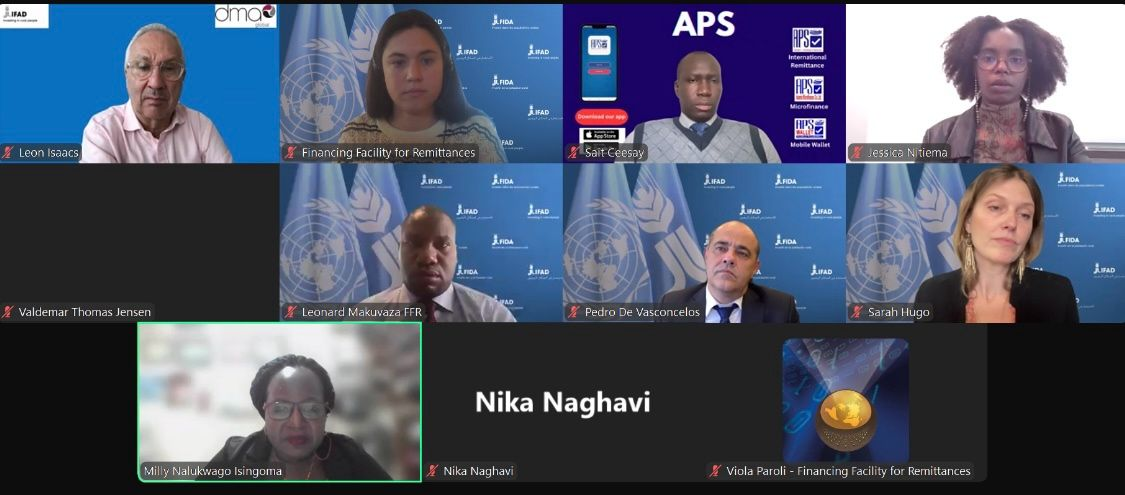
\includegraphics{images/1743167000666.jpg}

and in this
\href{https://www.linkedin.com/posts/financing-facility-for-remittances-ffr_remittance-activity-7311372331552014336-y1XR/}{LinkedIn
post}.

I eventually ran out of connection requests, which is probably for the
best, but these are people to potentially connect with. I am still
considering the best approach for outreach.

Other relevant people I found:

\begin{itemize}
\tightlist
\item
  \href{https://www.linkedin.com/in/leonisaacs/}{Leon Isaacs}
\item
  \href{https://www.linkedin.com/in/leonardmakuvaza/}{Leonard Makuvaza}
\item
  \href{https://www.linkedin.com/in/pedro-de-vasconcelos-899474a/}{Pedro
  de Vasconcelos}
\item
  \href{https://www.linkedin.com/in/sarah-hugo-794a853/}{Sarah Hugo}
\item
  \href{https://www.linkedin.com/posts/financing-facility-for-remittances-ffr_remittance-activity-7311372331552014336-y1XR/}{LinkedIn
  Remittance Activity Post}
\end{itemize}

\section{PDF Link}\label{pdf-link}

Here is the previous PDF link, which was previously not working:
\href{https://github.com/WilliamClintC/RER/blob/main/_output/8.pdf}{8.pdf}

\section{Found Remitscope Dataset}\label{found-remitscope-dataset}

During my research, I examined the Remitscope website in detail and
discovered raw data embedded within the website. While I am unsure if
this data is intended to be public, it was located deep within the site
code. The extracted files are saved in
\href{https://github.com/WilliamClintC/RER/tree/main/data/Remittance_3}{\texttt{data/Remittance\_3}}
.

\subsection{Remitscope Data analysis}\label{remitscope-data-analysis}

This is a quote from Remitscope

\begin{quote}
The World Bank has historically published estimates on remittance
inflows and outflows at a corridor level (in a bilateral matrix).
Estimated flows have been based on the number of migrants living in the
host country and an estimate on the amount they send home (based on the
income differential between the two countries). Whilst this data is
understood not to be as accurate and has since been removed from the
World Bank website, it is currently the best source available for this
data, which provides an indication of the relative value of flows across
corridors.
\end{quote}

\begin{itemize}
\tightlist
\item
  The central bank data is sparse; from central banks we have data for
  2020 to 2024, but many country pairs are missing compared to the World
  Bank dataset.
\item
  The World Bank data covers only 2021, but is much more detailed.
\item
  Currently, the dataset includes only African and Latin American
  countries. We need to decide whether this limited coverage is
  sufficient for our analysis.
\end{itemize}

To see a overview of the data see the following images:

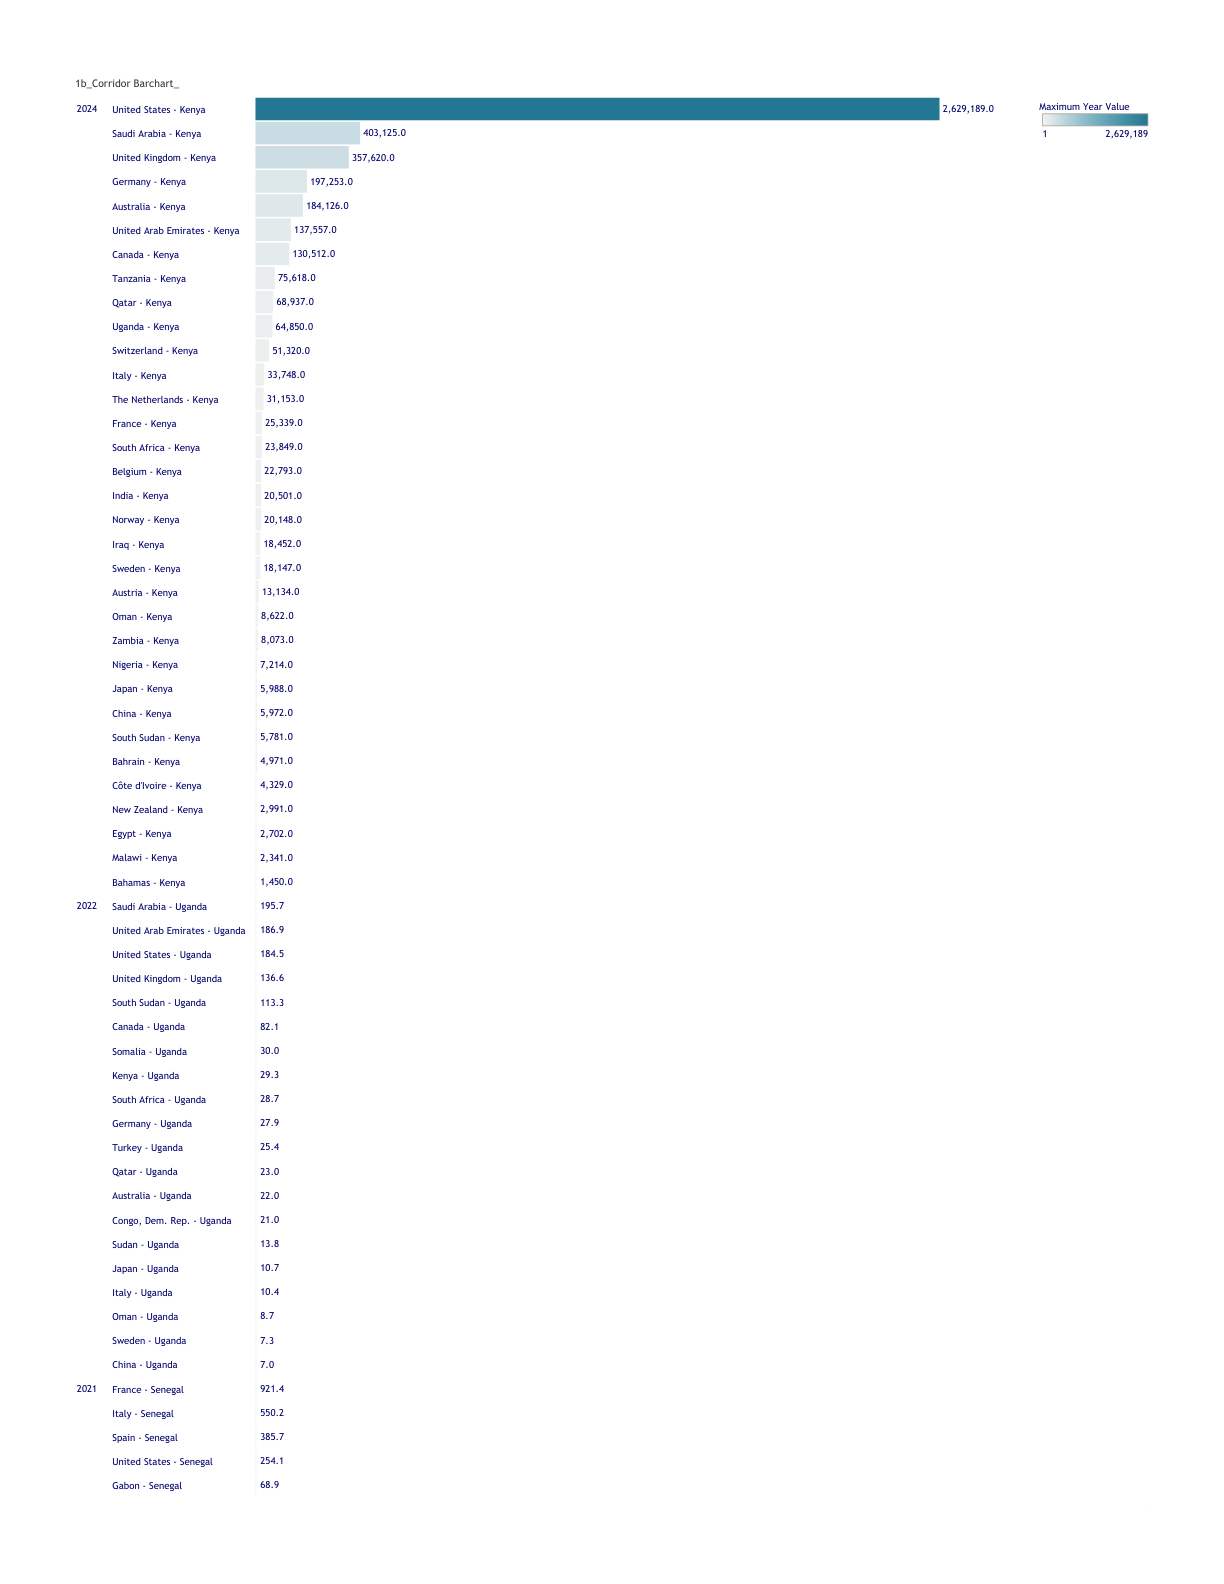
\includegraphics{data/Remittance_3/remitscope_africa_page_30.png}
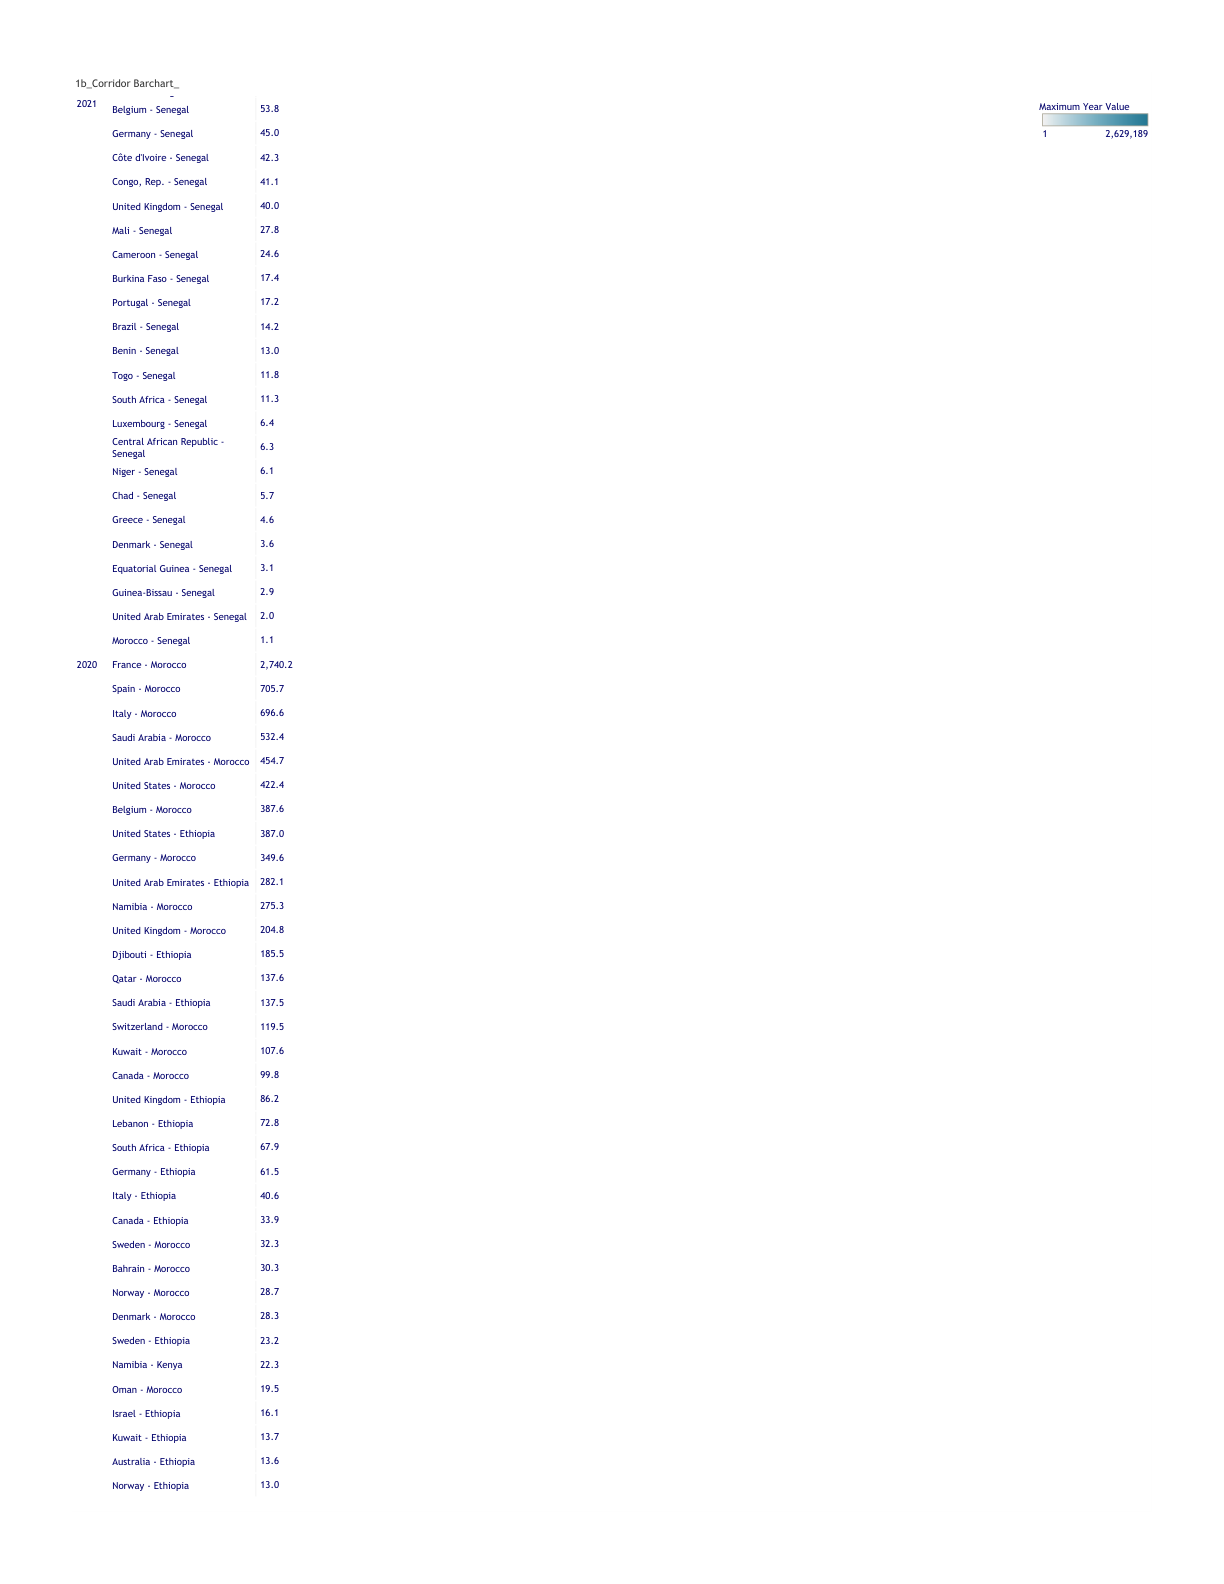
\includegraphics{data/Remittance_3/remitscope_africa_page_31.png}

\includegraphics{data/Remittance_3/remitscope_africa_page_32.png}
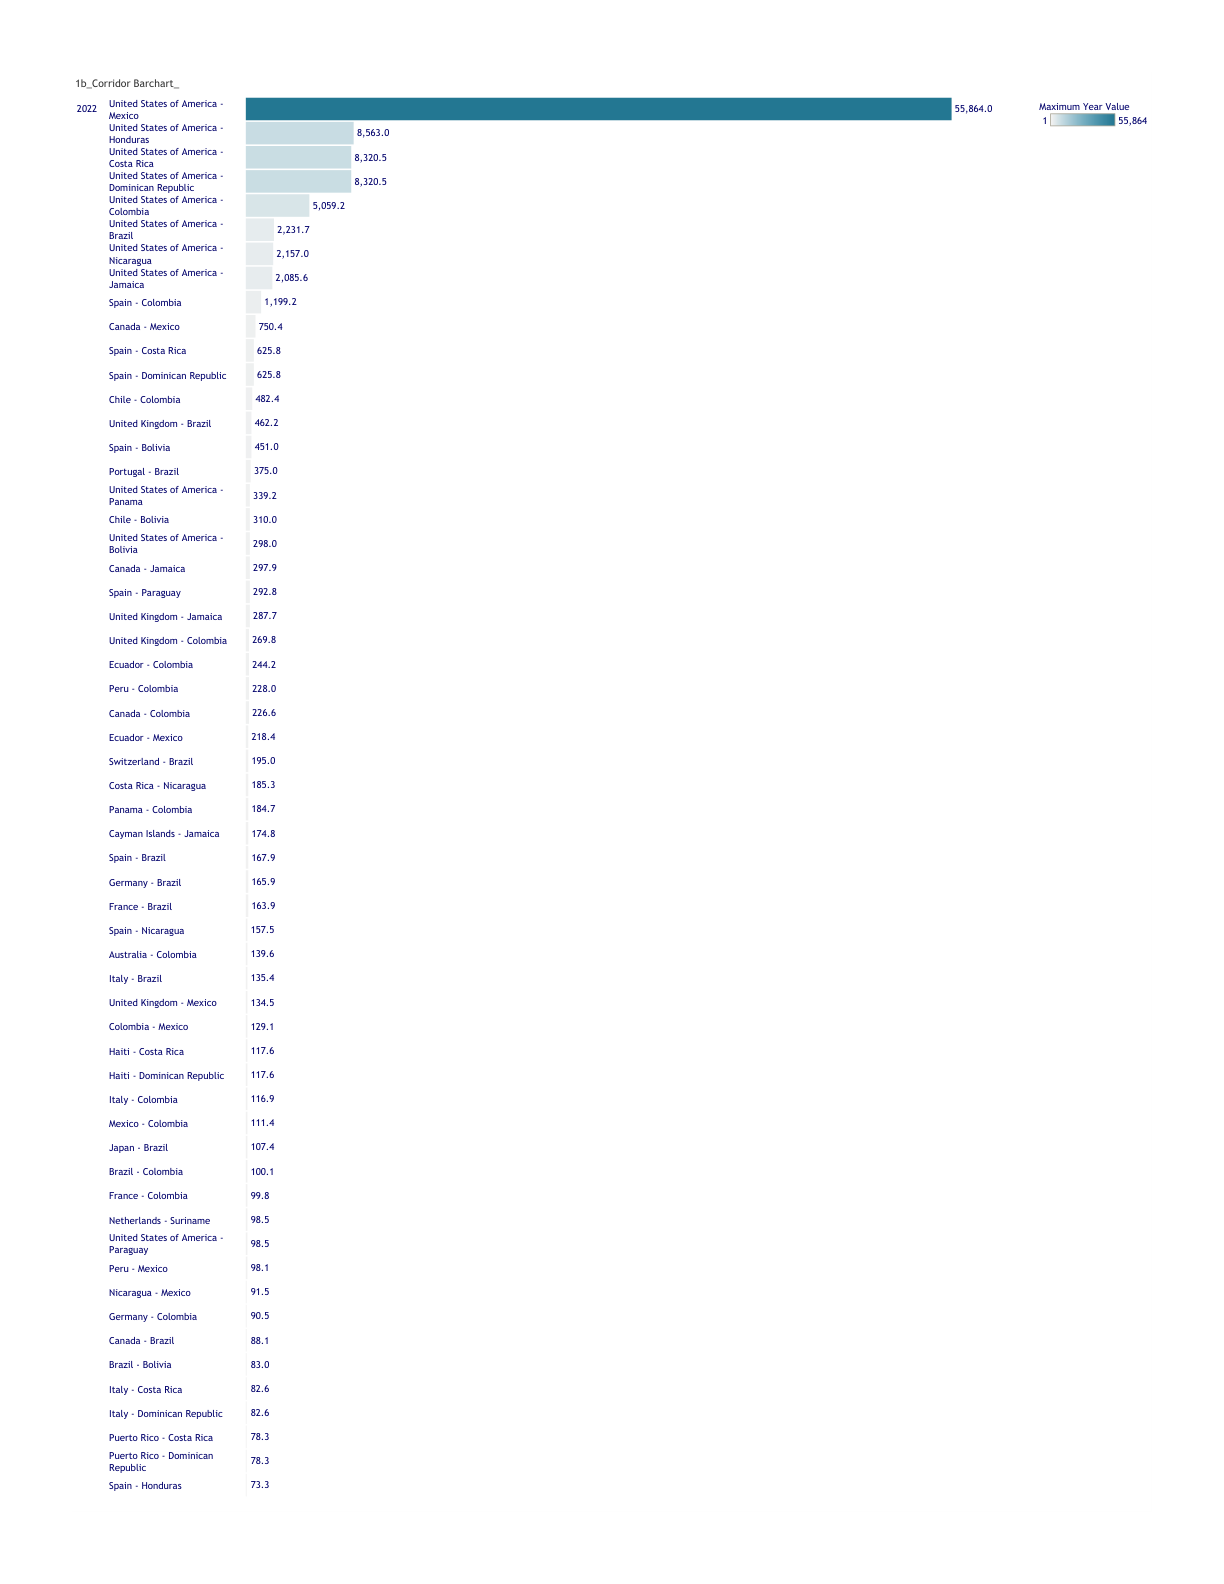
\includegraphics{data/Remittance_3/remitscope_page_36.png}
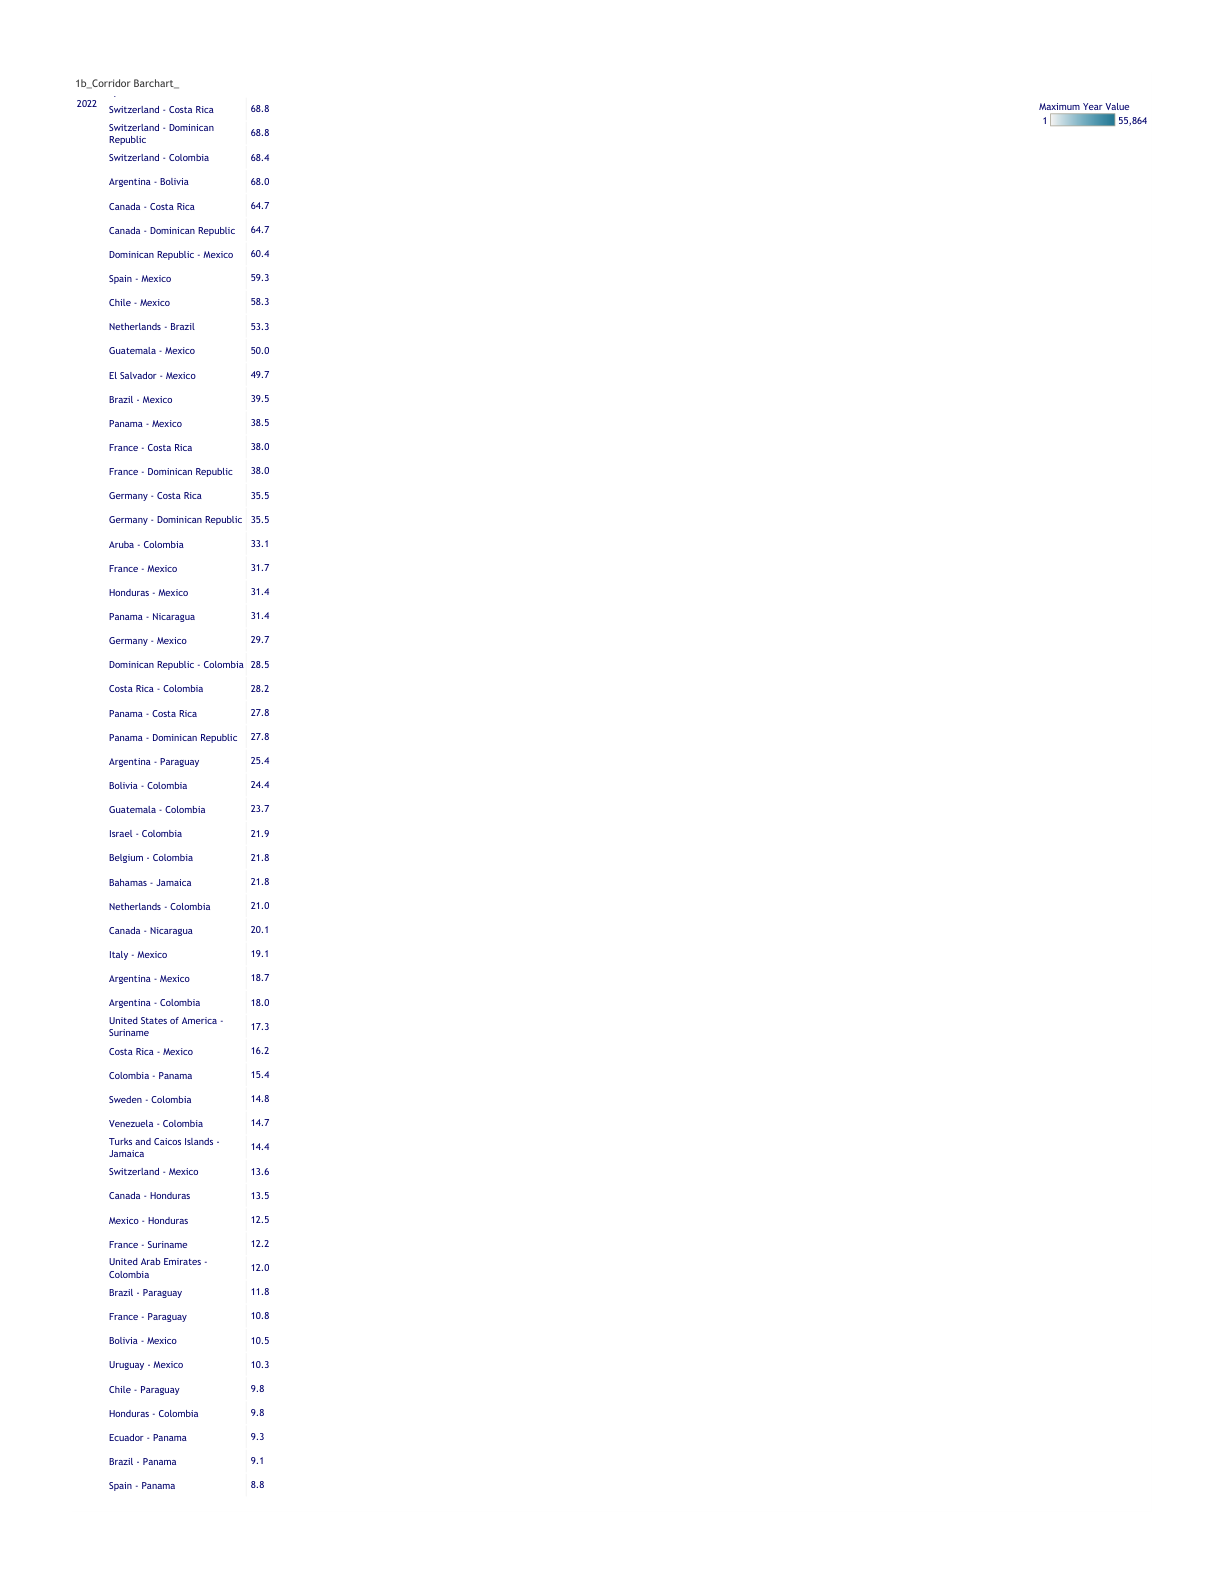
\includegraphics{data/Remittance_3/remitscope_page_37.png}
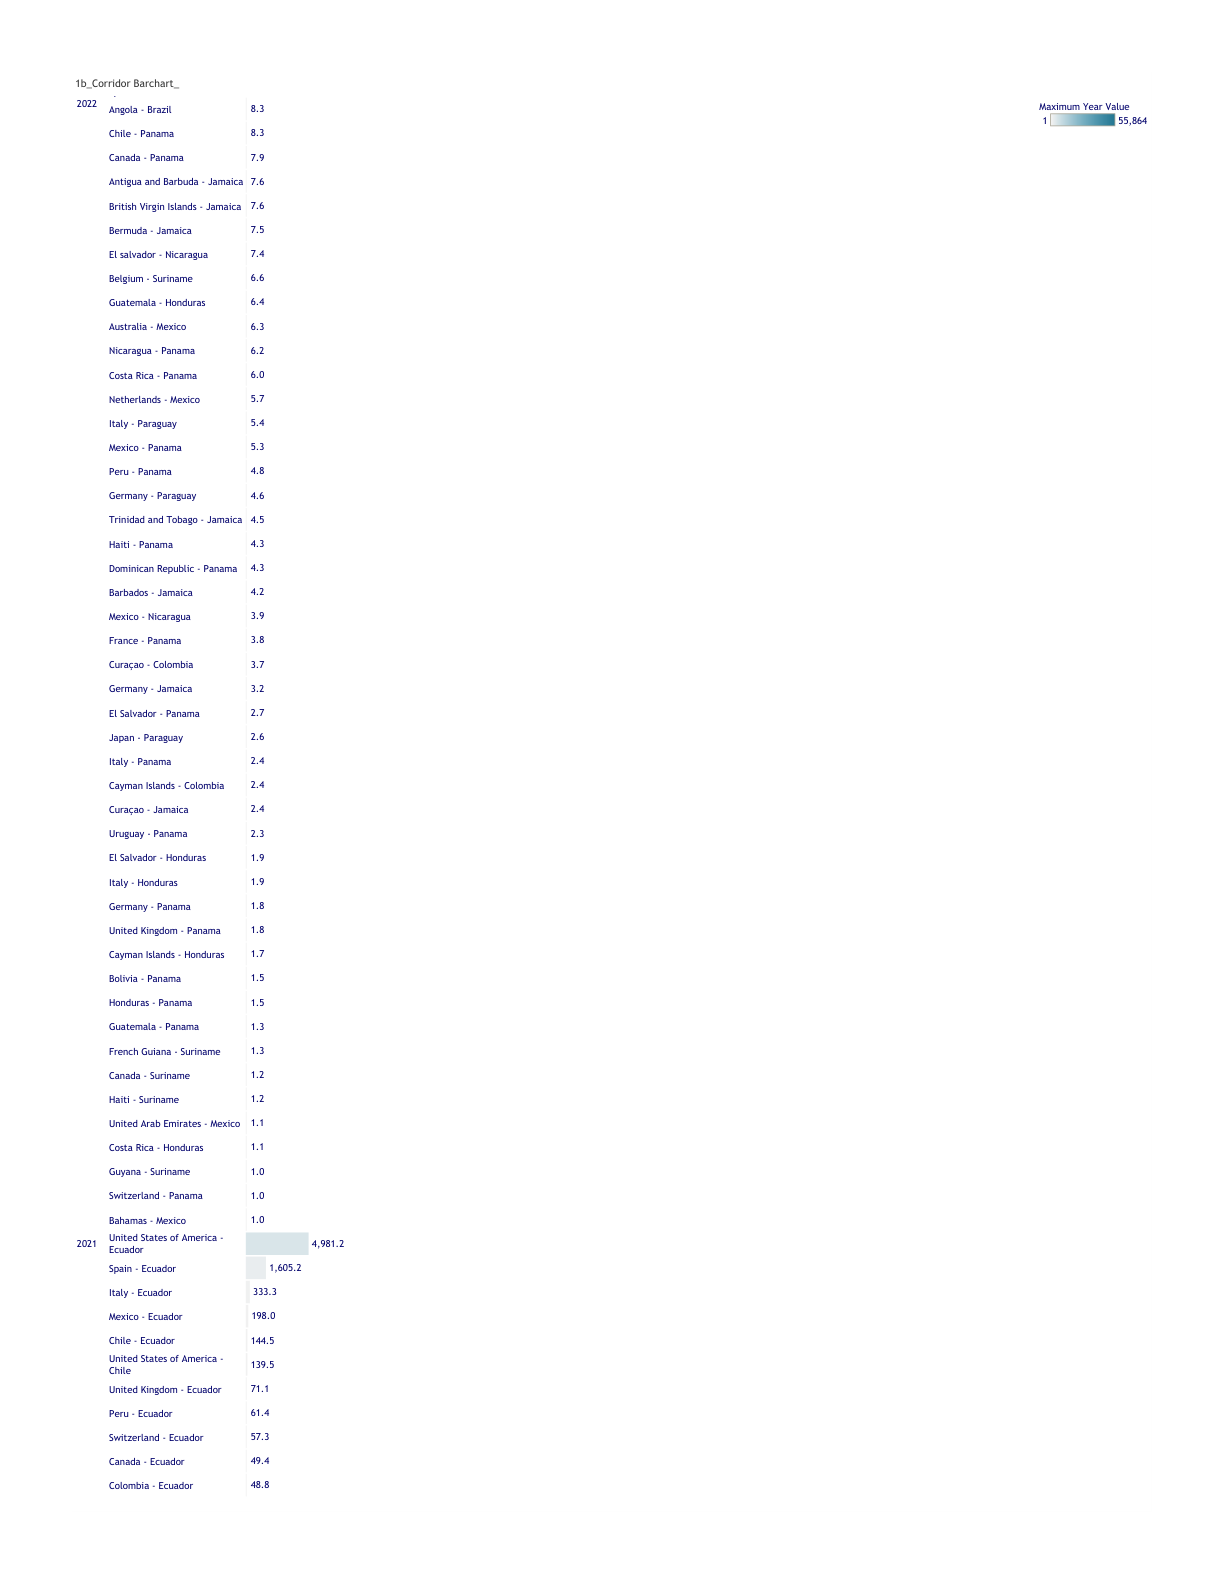
\includegraphics{data/Remittance_3/remitscope_page_38.png}
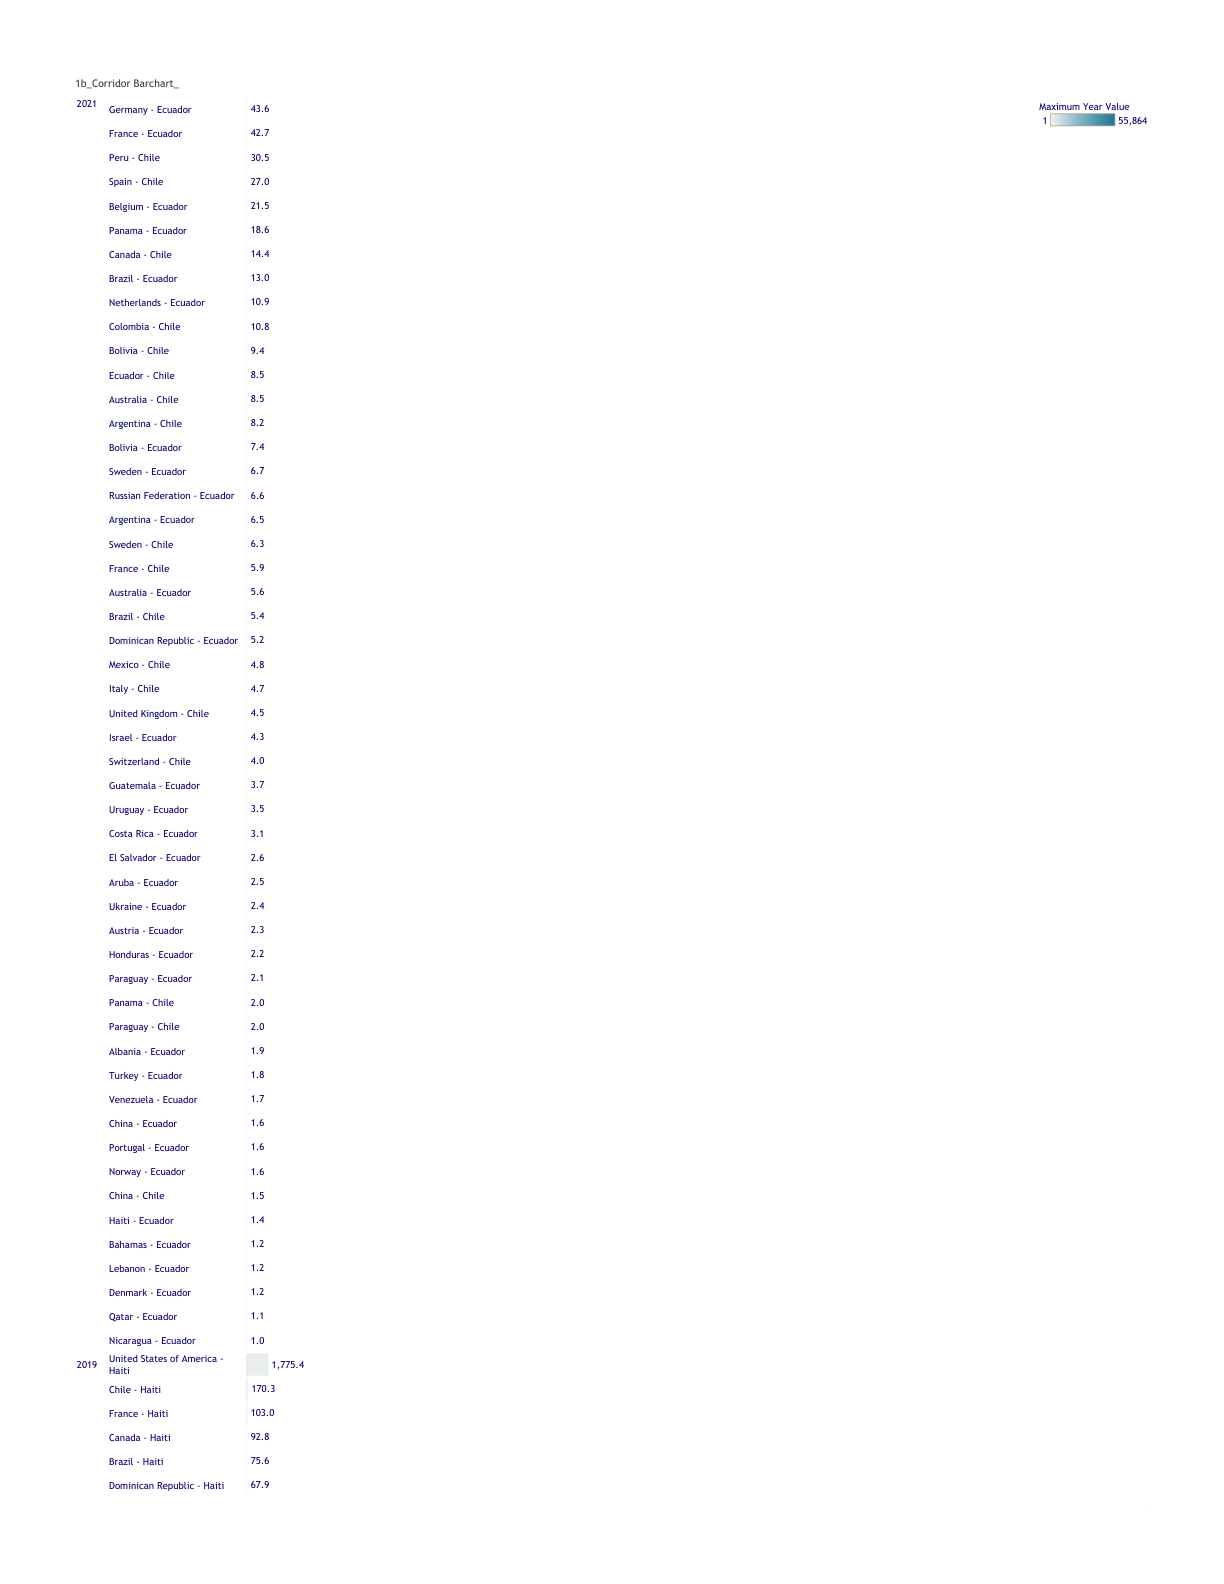
\includegraphics{data/Remittance_3/remitscope_page_39.png}

\includegraphics{data/Remittance_3/remitscope_page_40.png}

This is relatively limited compared to the world bank dataset.

\section{Clarification on Bitcoin}\label{clarification-on-bitcoin}

The challenge with analyzing Bitcoin transactions is that, while every
micro-level transaction is publicly observable, the wallets involved are
anonymized. As a result, we cannot directly determine the geographic
locations of the transactions.

\subsection{3 approaches}\label{approaches}

\subsubsection{Approach 1: Exchange
Wallets}\label{approach-1-exchange-wallets}

This is the initial approach, similar to what we would do with standard
fiat currency:

\begin{enumerate}
\def\labelenumi{\arabic{enumi}.}
\tightlist
\item
  We observe wallets.
\item
  We can determine where these wallets are based and construct the
  dataset shown below. Here, the \emph{exchanges} function as the
  ``banks'' in the traditional fiat system.
\end{enumerate}

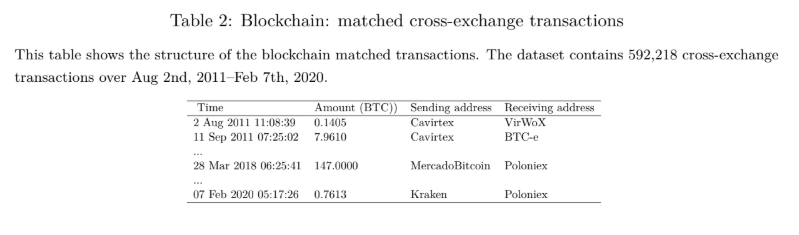
\includegraphics{images/Screenshot 2025-08-30 050944.png}

\begin{enumerate}
\def\labelenumi{\arabic{enumi}.}
\setcounter{enumi}{2}
\tightlist
\item
  The main limitation is that \emph{exchanges} are not bound by
  geography, which restricts this method. An exception is China, where
  the ``Great Firewall'' blocks access to foreign websites, requiring
  exchanges to be registered in China to serve Chinese users. This
  allows for a distinction between China-based and non-China-based
  exchanges, as done in
  \href{https://papers.ssrn.com/sol3/papers.cfm?abstract_id=3956933}{this
  link}.
\end{enumerate}

\subsubsection{Approach 2: Exchange Wallets and Web
Traffic}\label{approach-2-exchange-wallets-and-web-traffic}

\begin{enumerate}
\def\labelenumi{\arabic{enumi}.}
\tightlist
\item
  This approach builds on the limitations of Approach 1.
\item
  We can observe web traffic to the exchanges, including the geographic
  locations of the visitors. We also observe micro-transactions
  occurring across various exchanges.
\item
  Suppose there are two countries (Canada and China) and two exchanges
  (FTX and Binance):
\end{enumerate}

Suppose we observe a transaction of 100 BTC (Bitcoin), where a transfer
occurs from FTX to Binance.

Assume the users of FTX (the senders) are:

\begin{itemize}
\tightlist
\item
  50\% from Canada
\item
  50\% from China
\end{itemize}

And the users of Binance (the receivers) are:

\begin{itemize}
\tightlist
\item
  10\% in Canada
\item
  90\% in China
\end{itemize}

If 100 BTC is sent from FTX to Binance, the flows can be broken down as
follows:

\begin{itemize}
\tightlist
\item
  50 BTC leave Canada (100 BTC × 50\%)
\item
  50 BTC leave China (100 BTC × 50\%)
\item
  10 BTC arrive in Canada (100 BTC × 10\%)
\item
  90 BTC arrive in China (100 BTC × 90\%)
\end{itemize}

This can be further disaggregated:

\begin{itemize}
\tightlist
\item
  5 BTC: Canada to Canada (50 BTC × 10\%)
\item
  45 BTC: Canada to China (50 BTC × 90\%)
\item
  5 BTC: China to Canada (50 BTC × 10\%)
\item
  45 BTC: China to China (50 BTC × 90\%)
\end{itemize}

The net flow is:

\begin{itemize}
\tightlist
\item
  45 BTC from Canada to China
\item
  5 BTC from China to Canada
\end{itemize}

\paragraph{Assumptions}\label{assumptions}

\begin{enumerate}
\def\labelenumi{\arabic{enumi}.}
\setcounter{enumi}{3}
\tightlist
\item
  Key assumption:

  \begin{enumerate}
  \def\labelenumii{\arabic{enumii}.}
  \tightlist
  \item
    users do not mask online activity by employing virtual private
    networks (VPNs)
  \item
    transaction amounts are, on average, broadly equal across users in
    different countries
  \item
    These assumptions are similar to those used by the IMF when
    estimating remittances based on population shares.

    \begin{enumerate}
    \def\labelenumiii{\arabic{enumiii}.}
    \tightlist
    \item
      For example, suppose we observe remittances in Canada, where the
      immigrant population is 50\% from China and 50\% from the
      Philippines. If total remittances are \$100 CAD, we would
      attribute \$50 CAD to China and \$50 CAD to the Philippines,
      reflecting the 50\% immigrant profile.
    \item
      In this IMF example, the key assumption is that transaction
      amounts are uniform across each individual (similar to the bitcoin
      assumption)
    \end{enumerate}
  \end{enumerate}
\end{enumerate}

\subsubsection{Approach 3: Fiat
Currencies}\label{approach-3-fiat-currencies}

\begin{enumerate}
\def\labelenumi{\arabic{enumi}.}
\tightlist
\item
  peer-to-peer exchange called LocalBitcoins: an escrow service for
  Bitcoin transactions.
\item
  When people want to trade Bitcoin, they use LocalBitcoins to exchange
  Bitcoin for fiat currency.
\item
  These transactions are observable: we can see the amount of BTC sold
  and the amount of fiat currency exchanged. We can not observe the
  wallets.
\item
  The key innovation is because Bitcoin transactions are public,
  researchers look for transactions of the same size and timeframe to
  link wallets with the fiat currency transaction.
\item
  For example, suppose an individual buys Bitcoin with Philippine pesos
\item
  LocalBitcoins records a transaction of 1.000003 BTC for 6 million
  pesos on August 31st at 2:00 PM.
\item
  Using the developed algorithm, it searches for a matching 1.000003 BTC
  transaction on the public blockchain.
\item
  Once found, the anonymized wallet involved in the transaction can be
  observed and associated with the Philippines and Philippine pesos.
\item
  Next, suppose someone sells 1.000003 BTC for 150,000 CAD in Canada at
  2:30 PM on the same day.
\item
  The algorithm repeats the process, associating the wallet with both
  the Philippines and Canada.
\item
  In this way, a cross-border transfer is identified and recorded,
  Philippines to Canada cross border flow.
\end{enumerate}

\paragraph{Assumptions}\label{assumptions-1}

\begin{enumerate}
\def\labelenumi{\arabic{enumi}.}
\setcounter{enumi}{5}
\tightlist
\item
  Key Assumptions:
\item
  The probability of observing two transactions of the same size within
  a 5-hour period is low.
\item
  People are risk-averse and minimize bitcoin volatility by immediately
  trading it.
\item
  LocalBitcoins is representative of broader crypto cross-border flows.
\end{enumerate}

More detail can be found in
\href{https://www.ecb.europa.eu/pub/pdf/scpwps/ecb.wp2868~0c2ad2e6e7.en.pdf}{this
paper}.

\subsection{Stablecoin Flows Paper}\label{stablecoin-flows-paper}

A recent paper,
\href{https://www.imf.org/en/Publications/WP/Issues/2025/07/11/Decrypting-Crypto-How-to-Estimate-International-Stablecoin-Flows-568260}{Decrypting
Crypto: How to Estimate International Stablecoin Flows} (IMF, 2025)

\begin{enumerate}
\def\labelenumi{\arabic{enumi}.}
\tightlist
\item
  The study analyzes stablecoin flows by integrating transaction data
  with exchange locations, timing of activity, and geographic patterns
  to infer wallet origins.
\item
  It leverages user-assigned domain names (e.g., ``Pierre'') as
  identifiers, providing additional context beyond anonymized wallet
  strings.
\item
  AI models combine domain names with transaction timing to estimate
  user locations for instance, a wallet named ``Pierre'' active during
  France business hours is probabilistically associated with Europe.
\item
  The model also incorporates data from region-specific exchanges. An
  example would be suppose we observe a wallet interacting with
  Coinhouse, a Paris-based crypto exchange, with a domain name
  ``Pierre'' combined with France time trading behavior. This
  information would associate the wallet with a high probability to
  Europe.
\item
  Unlike most prior work, which emphasizes stablecoins as hedges against
  U.S. dollar instability, this paper highlights their significance in
  facilitating cross-border flows.
\end{enumerate}

Key findings from the paper include:

\begin{quote}
In absolute terms, Asia and the Pacific lead with the highest stablecoin
activity (inflows: \$407bn, outflows: \$395bn, intraregional flows:
\$209bn), followed by North America (inflows: \$363bn, outflows:
\$417bn, intraregional flows: \$216bn). However, relative to GDP, Africa
and the Middle East, and Latin America and the Caribbean stand out, with
stablecoin usage reaching 6.7\% and 7.7\% of GDP, respectively.
\end{quote}

\begin{quote}
Calculating bilateral net flows highlights North America as the primary
source of stablecoin outflows into all other regions of the world,
estimated at \$54bn in 2024. The data show that net stablecoin flows
from North America to other regions increase when domestic currencies
are weak.
\end{quote}

\begin{quote}
This suggests that stablecoins could increasingly serve as an instrument
to meet global demand for dollars, particularly in regions where access
to traditional dollar markets is constrained.
\end{quote}

\begin{quote}
Stablecoins are typically minted in the U.S., where issuers convert fiat
dollars into digital tokens. The analysis shows that stablecoin net
flows are largely outflows from North America. The authors hypothesize
that these net outflows are linked to global demand for U.S. dollars,
especially when local currencies depreciate.
\end{quote}

\subsubsection{Dataset Discrepancies}\label{dataset-discrepancies}

Big discrepancies between the various methodologies, possibly because of
VPN. \textgreater{} For 2024, we estimate 5.5 times more gross
stablecoin flows involving China (i.e., \$153bn vs \$28bn) and 100 times
more net flows of stablecoins into China (i.e., \$18bn vs \$0.18bn)

\section{Appendix}\label{appendix}

\subsection{IMF External Sector
Report}\label{imf-external-sector-report}

For further reading, see the
\href{https://www.imf.org/-/media/Files/Publications/ESR/2025/English/ch2.ashx?utm_source}{IMF
External Sector Report (2025, Chapter 2)}.


\printbibliography


\end{document}
